\documentclass[10pt,a4paper,twocolumn]{article}

\usepackage{amsmath,amssymb}
\usepackage{graphicx}
\usepackage{booktabs}
\usepackage{array}
\usepackage{multirow}
\usepackage[colorlinks=true,linkcolor=blue,citecolor=blue,urlcolor=blue]{hyperref}
\usepackage{caption}
\usepackage{subcaption}
\usepackage{natbib}
\usepackage[top=1in,bottom=1in,left=0.75in,right=0.75in,columnsep=0.25in]{geometry}
\usepackage{microtype}

\title{\textbf{Beyond Binary: Four-Class Risk Stratification from\\
Gastrointestinal Endoscopy Using Asymmetric-Cost\\
Lightweight CNN--Transformer Learning\\
and Demographic Equity Analysis}}

\author{Azizur Rahman\\
\small Department of Computer Science, Indiana Wesleyan University, Marion, IN 46953, USA\\
\small RadTH Technologies\\
\small \texttt{azizurusa22@gmail.com}}

\date{}

\begin{document}

\twocolumn[{%
\maketitle
\begin{@twocolumnfalse}
\begin{abstract}
Gastrointestinal (GI) cancers account for over 3.5 million deaths annually,
yet existing AI-assisted endoscopy systems reduce the clinical decision to a
binary lesion-present/absent output that is misaligned with actionable
clinical practice guidelines and provides no guidance on intervention urgency.
We present the first lightweight CNN--Transformer benchmark for four-class GI
lesion \emph{risk stratification} aligned with American College of
Gastroenterology (ACG) and European Society of Gastrointestinal Endoscopy
(ESGE) guidelines. We map 23 HyperKvasir finding classes to four clinically
actionable risk tiers---Normal (routine surveillance), Inflammatory (medical
management), Pre-malignant (biopsy required), and High-Risk (immediate
intervention)---and train three lightweight architectures (DenseNet-121,
EfficientNet-B0, DeiT-Tiny; all $<$8\,M parameters) under a novel
\textbf{Asymmetric Endoscopy Loss (AEL)} that assigns a 5$\times$
misclassification penalty to High-Risk lesions, reflecting the clinical
reality that missed High-Risk lesions reduce five-year survival from 90\% to
under 20\%. Contrast-Limited Adaptive Histogram Equalisation (CLAHE)
preprocessing enhances mucosal contrast prior to augmentation. Cross-dataset
generalisation is validated zero-shot on the independent Kvasir-v2 cohort.
GradCAM heatmaps localise clinically relevant mucosal features per risk tier,
Monte Carlo Dropout uncertainty quantification flags borderline cases for
mandatory endoscopist review, and a Cross-Demographic Consistency of
Tier-level Equity Index (CD-CTEI) assesses model fairness across age and sex
subgroups. The best model reaches macro F1\,$=$\,[TBD] on HyperKvasir and
[TBD] zero-shot on Kvasir-v2, with [TBD]\,\% workload reduction and zero
missed High-Risk cases.
\end{abstract}

\noindent\textbf{Keywords:}
Gastrointestinal endoscopy;
Risk stratification;
Asymmetric loss function;
Lightweight neural networks;
Vision Transformer;
DenseNet;
EfficientNet;
GradCAM;
Monte Carlo Dropout;
Clinical equity;
HyperKvasir
\end{@twocolumnfalse}
}]

\bigskip

%% ============================================================================
\section{Introduction}
\label{sec:intro}
%% ============================================================================

Gastrointestinal cancers---encompassing colorectal, gastric, and oesophageal
malignancies---collectively account for more than 3.5 million deaths annually
and represent the second leading cause of cancer mortality
worldwide~\citep{Sung2021}. Early-stage lesions are missed in up to 26\,\% of
endoscopic procedures due to subtle mucosal changes, inter-endoscopist
variability, and endoscopist fatigue during high-volume screening
sessions~\citep{Kaminski2017}. Computer-aided detection (CAD) systems have
demonstrated statistically significant improvements in polyp detection in
randomised controlled trials~\citep{Wang2019}, leading to regulatory approval
of the first AI endoscopy devices. However, the clinical utility of deployed
CAD systems remains constrained by a fundamental design mismatch: virtually
all systems reduce the endoscopic decision to a binary lesion-present or
lesion-absent output~\citep{Pogorelov2017}.

This binary framing does not correspond to any published clinical practice
guideline. Both the ACG and the ESGE classify GI findings into tiered risk
categories that map to distinct clinical actions: routine surveillance
intervals for normal mucosa, medical management for inflammatory lesions,
mandatory biopsy and intensified surveillance for pre-malignant findings, and
immediate endoscopic resection or oncology referral for high-risk
lesions~\citep{Shaukat2021,Ferlitsch2017}. A binary AI output cannot guide
these decisions, reducing the technology to a simple alert with no actionable
resolution. Furthermore, binary systems apply identical classification costs
to all errors, ignoring the critical asymmetry in clinical consequences: a
missed High-Risk lesion may progress to invasive cancer within months, while
over-triaging a Normal finding results only in an unnecessary repeat
procedure~\citep{Rawla2019}.

Prior deep learning work on GI endoscopy has focused predominantly on polyp
detection~\citep{Tajbakhsh2016} and binary lesion
classification~\citep{Pogorelov2017}. Multi-class staging has been explored
in isolated contexts, such as Barrett's oesophagus severity
grading~\citep{Ebigbo2019}, but no prior work has framed the problem as a
unified four-class risk stratification aligned with ACG/ESGE guidelines
across the entire GI tract. Compact Vision Transformers, specifically
DeiT-Tiny~\citep{Touvron2021} with 5.9\,M parameters, enable global mucosal
context modelling through patch token self-attention without the 86\,M$+$
parameter cost of full ViT~\citep{Dosovitskiy2021}, making them deployable on
clinical-grade hardware. On the loss side, Focal Loss~\citep{Lin2017}
addresses class imbalance by down-weighting easy examples but does not encode
inter-class \emph{risk} asymmetry---the clinically critical distinction
between missing a Normal finding and missing a High-Risk lesion.

We address these limitations by framing GI endoscopy AI as a \emph{four-class
risk stratification problem} directly aligned with ACG/ESGE guidelines. Our
specific contributions are:
\begin{enumerate}
  \item A clinically grounded four-class risk schema mapping 23 HyperKvasir
        finding classes to actionable intervention tiers;
  \item A novel \textbf{Asymmetric Endoscopy Loss (AEL)} encoding the clinical
        cost asymmetry between risk tiers, with a 5$\times$ penalty weight on
        High-Risk misclassification;
  \item The first lightweight CNN--Transformer benchmark ($<$8\,M parameters)
        for this four-class task, comparing DenseNet-121, EfficientNet-B0, and
        DeiT-Tiny under identical training conditions;
  \item Cross-dataset zero-shot evaluation on Kvasir-v2 to assess
        generalisation to unseen populations and imaging equipment;
  \item GradCAM explainability localising clinically meaningful features per
        risk tier for both CNN and Transformer architectures;
  \item Monte Carlo Dropout uncertainty quantification enabling a risk-adaptive
        referral protocol with zero missed High-Risk lesions by design;
  \item An AEL ablation against standard cross-entropy and Focal Loss; and
  \item A Cross-Demographic Consistency of Tier-level Equity Index (CD-CTEI)
        assessing prediction fairness across age and sex subgroups.
\end{enumerate}

%% ============================================================================
\section{Methods}
\label{sec:methods}
%% ============================================================================

\subsection{Datasets}
\label{sec:datasets}

We used HyperKvasir~\citep{Borgli2020} as the primary training and evaluation
dataset. HyperKvasir is the largest publicly available annotated GI endoscopy
dataset, comprising 110,079 images from both upper and lower GI tract
examinations collected at Baerum Hospital, Norway. The labelled image subset
contains 10,662 images across 23 finding classes, organised in a nested
directory structure by GI tract region, anatomical category, and finding
class. Each class folder contains JPEG images of variable resolution,
standardised to $224\times224$ pixels prior to training.

For external validation, we used Kvasir-v2~\citep{Pogorelov2017b}, an
independent dataset of 8,000 images across 8 GI finding classes collected
from a different patient population and imaging equipment. Kvasir-v2 was used
exclusively for zero-shot evaluation---no Kvasir-v2 images were used during
training or hyperparameter selection. This design tests the ability of models
trained on HyperKvasir to generalise to a clinically and technically distinct
cohort.

The full dataset was split at the image level with stratified sampling into
training (70\%), validation (15\%), and test (15\%) sets, with reproducibility
ensured by a fixed random seed (SEED\,$=$\,42). The training set was further
balanced using \texttt{WeightedRandomSampler} with weights inversely
proportional to class frequencies, ensuring equal expected class
representation per batch.

Figure~\ref{fig:samples} shows representative images from each risk tier in
both datasets, illustrating the visual diversity within each class and the
appearance difference between imaging systems. Figure~\ref{fig:dist} shows
the class distribution in both datasets after mapping to the four-tier schema,
confirming class imbalance in HyperKvasir and motivating the use of
WeightedRandomSampler and macro F1 as the primary evaluation metric.

\begin{figure*}[htbp]
  \centering
  \begin{subfigure}[b]{0.48\textwidth}
    
\includegraphics[width=\linewidth]{samples_hyperkvasir.png}
    \caption{HyperKvasir (training dataset)}
  \end{subfigure}
  \hfill
  \begin{subfigure}[b]{0.48\textwidth}
    \includegraphics[width=\linewidth]{"samples_kvasir-v2.png"}
    \caption{Kvasir-v2 (zero-shot evaluation dataset)}
  \end{subfigure}
  \caption{Representative endoscopy images per risk tier from both datasets.
    Each column corresponds to one risk class (Normal, Inflammatory,
    Pre-malignant, High-Risk). Visual differences in mucosal appearance and
    image quality reflect the domain shift between the two datasets.}
  \label{fig:samples}
\end{figure*}

\begin{figure*}[htbp]
  \centering
  \begin{subfigure}[b]{0.48\textwidth}
    \includegraphics[width=\linewidth]{"dist_hyperkvasir_—_class_distribution.png"}
    \caption{HyperKvasir class distribution}
  \end{subfigure}
  \hfill
  \begin{subfigure}[b]{0.48\textwidth}
    \includegraphics[width=\linewidth]{"dist_kvasir-v2_—_class_distribution.png"}
    \caption{Kvasir-v2 class distribution}
  \end{subfigure}
  \caption{Risk-tier class distributions after ACG/ESGE schema mapping.
    HyperKvasir shows pronounced class imbalance, motivating
    WeightedRandomSampler and macro F1 as the primary metric. Kvasir-v2
    has a different distribution, reflecting a realistic cross-site
    deployment scenario.}
  \label{fig:dist}
\end{figure*}

\subsection{Clinical Risk Schema}
\label{sec:schema}

We defined a four-class risk stratification schema by mapping the 23
HyperKvasir finding classes to clinically actionable risk tiers based on ACG
and ESGE clinical practice guidelines~\citep{Shaukat2021,Ferlitsch2017}. The
mapping is shown in Table~\ref{tab:schema}. Two HyperKvasir classes
(\texttt{bbps-0-1}, \texttt{impacted-stool}) were excluded as they represent
bowel preparation quality scores and non-pathological states without clinical
risk stratification relevance, yielding 21 usable finding classes across the
four tiers.

\begin{table*}[htbp]
\centering
\caption{Four-class clinical risk stratification schema (ACG/ESGE
  guideline-aligned).}
\label{tab:schema}
\begin{tabular}{clp{4.2cm}p{4.2cm}}
\toprule
\textbf{Class} & \textbf{Label} & \textbf{HyperKvasir Source Classes} &
\textbf{Clinical Action}\\
\midrule
0 & Normal &
  \texttt{cecum}, \texttt{pylorus}, \texttt{z-line},
  \texttt{retroflex-stomach}, \texttt{retroflex-rectum}, \texttt{ileum},
  \texttt{bbps-2-3} &
  Routine surveillance (5--10\,yr interval)\\[4pt]
1 & Inflammatory &
  \texttt{esophagitis-a}, \texttt{ulcerative-colitis-grade-0-1},
  \texttt{ulcerative-colitis-grade-1}, \texttt{hemorrhoids} &
  Medical management + annual follow-up\\[4pt]
2 & Pre-malignant &
  \texttt{barretts}, \texttt{barretts-short-segment},
  \texttt{esophagitis-b-d}, \texttt{polyps},
  \texttt{ulcerative-colitis-grade-1-2},
  \texttt{ulcerative-colitis-grade-2} &
  Mandatory biopsy + 3--6\,month surveillance\\[4pt]
3 & High-Risk &
  \texttt{ulcerative-colitis-grade-2-3},
  \texttt{ulcerative-colitis-grade-3},
  \texttt{dyed-lifted-polyps},
  \texttt{dyed-resection-margins} &
  Immediate resection / oncology referral\\
\bottomrule
\end{tabular}
\end{table*}

\subsection{Image Preprocessing and Augmentation}
\label{sec:preproc}

Endoscopic images frequently exhibit non-uniform illumination and low mucosal
contrast. We applied Contrast-Limited Adaptive Histogram Equalisation
(CLAHE)~\citep{Reza2004} to the L-channel of each image in CIE L*a*b* colour
space, with clip limit 2.0 and tile grid size $8\times8$. CLAHE enhances
local contrast in mucosal texture and vascular architecture while the clip
limit prevents noise amplification in over-bright regions.

Training augmentation comprised: random horizontal flip ($p=0.5$), random
vertical flip ($p=0.2$), random rotation ($\pm15^{\circ}$), and colour
jitter (brightness\,$=$\,0.2, contrast\,$=$\,0.2, saturation\,$=$\,0.1).
Validation and test images received only CLAHE preprocessing followed by
resize to $224\times224$ pixels. All images were normalised using ImageNet
population statistics ($\mu=[0.485, 0.456, 0.406]$,
$\sigma=[0.229, 0.224, 0.225]$).

\subsection{Model Architectures}
\label{sec:models}

We benchmarked three lightweight architectures, each with fewer than 8\,M
parameters, representing two computational paradigms: convolutional networks
(DenseNet-121, EfficientNet-B0) and a compact Vision Transformer (DeiT-Tiny).
All models are pre-trained on ImageNet-1k and fine-tuned with task-specific
classification heads (Table~\ref{tab:archs}).

\begin{table*}[htbp]
\centering
\caption{Lightweight model architectures benchmarked (all $<$8\,M parameters).}
\label{tab:archs}
\begin{tabular}{lccccc}
\toprule
\textbf{Model} & \textbf{Type} & \textbf{Pre-training} &
\textbf{Parameters} & \textbf{Input} & \textbf{Head Dropout}\\
\midrule
DenseNet-121    & CNN         & ImageNet-1k & 7.0\,M & $224^2$ & 0.5\\
EfficientNet-B0 & CNN         & ImageNet-1k & 5.3\,M & $224^2$ & 0.3\\
DeiT-Tiny       & Transformer & ImageNet-1k & 5.9\,M & $224^2$ & 0.1\\
\bottomrule
\end{tabular}
\end{table*}

\textbf{DenseNet-121}~\citep{Huang2017} employs dense connectivity in which
each layer receives feature maps from all preceding layers, promoting feature
reuse. Its classification head is Dropout(0.5)\,$\to$\,Linear($1024\!\to\!4$).

\textbf{EfficientNet-B0}~\citep{Tan2019} applies compound scaling of depth,
width, and resolution jointly. Its head is
Dropout(0.3)\,$\to$\,Linear($1280\!\to\!256$)\,$\to$\,ReLU\,$\to$\,
Dropout(0.2)\,$\to$\,Linear($256\!\to\!4$).

\textbf{DeiT-Tiny}~\citep{Touvron2021} processes $224\times224$ images as
196 non-overlapping $16\times16$ patch tokens through 12 self-attention
layers. Its head appends Dropout(0.1)\,$\to$\,Linear($192\!\to\!4$) to the
class token. Dropout rates are calibrated to model capacity; the dense CNN
requires stronger regularisation while the Transformer benefits from lighter
dropout due to implicit regularisation through the attention mechanism.

\subsection{Asymmetric Endoscopy Loss}
\label{sec:ael}

Standard cross-entropy assigns equal cost to all misclassifications. In GI
risk stratification this is clinically inappropriate: a missed High-Risk
lesion may progress to invasive cancer, reducing five-year survival from
over 90\,\% for stage~I disease to under 20\,\% for
stage~IV~\citep{Sung2021}. We propose the \textbf{Asymmetric Endoscopy Loss
(AEL)}, a weighted cross-entropy formulation:

\begin{equation}
  \mathcal{L}_{\text{AEL}}(\hat{y}, y) =
    \text{CrossEntropy}(\hat{y},\, y;\, \mathbf{w}), \quad
  \mathbf{w} = [1.0,\; 3.5,\; 3.0,\; 5.0]
  \label{eq:ael}
\end{equation}

The weight vector $\mathbf{w}$ encodes the relative clinical cost of
misclassifying each risk tier (Table~\ref{tab:ael_weights}). The asymmetric
ratio 5:1 between High-Risk and Normal is consistent with published GI
oncology mortality data~\citep{Rawla2019}.

\begin{table*}[htbp]
\centering
\caption{AEL class weight rationale.}
\label{tab:ael_weights}
\begin{tabular}{clr p{9cm}}
\toprule
\textbf{Class} & \textbf{Label} & \textbf{Weight} &
\textbf{Clinical consequence of misclassification}\\
\midrule
0 & Normal        & 1.0 & Unnecessary repeat surveillance only\\
1 & Inflammatory  & 3.5 & Delayed medical treatment; mucosal progression\\
2 & Pre-malignant & 3.0 & Missed biopsy; unmonitored malignant transformation\\
3 & High-Risk     & 5.0 & Missed intervention; preventable cancer mortality\\
\bottomrule
\end{tabular}
\end{table*}

\subsection{Training Protocol}
\label{sec:training}

All models were trained for 25 epochs using the AdamW
optimiser~\citep{Loshchilov2019} with initial learning rate
$2\!\times\!10^{-4}$ and weight decay $1\!\times\!10^{-4}$. The learning
rate was annealed using CosineAnnealingLR with
$\eta_{\min}=1\!\times\!10^{-6}$. Gradient norms were clipped at 1.0. Batch
size was 32 for all models. A fixed random seed (SEED\,$=$\,42) was applied
with \texttt{cudnn.deterministic=True} for reproducibility. The best
checkpoint per model was saved based on validation macro F1-score. Training
was conducted on Apple M2 Metal Performance Shaders (MPS) hardware.
Hyperparameters are summarised in Table~\ref{tab:hparams}.

\begin{table}[htbp]
\centering
\caption{Training hyperparameters (identical for all three models).}
\label{tab:hparams}
\begin{tabular}{ll}
\toprule
\textbf{Hyperparameter} & \textbf{Value}\\
\midrule
Optimiser          & AdamW\\
Learning rate      & $2\times10^{-4}$\\
Weight decay       & $1\times10^{-4}$\\
LR schedule        & CosineAnnealingLR ($\eta_{\min}=1\times10^{-6}$)\\
Epochs             & 25\\
Batch size         & 32\\
Gradient clipping  & 1.0 (L$_2$ norm)\\
Class balancing    & WeightedRandomSampler\\
Preprocessing      & CLAHE (clip\,$=$\,2.0, tile\,$=$\,$8\times8$)\\
Reproducibility    & SEED\,$=$\,42, \texttt{cudnn.deterministic=True}\\
\bottomrule
\end{tabular}
\end{table}

Figure~\ref{fig:training} shows training and validation loss and macro
F1-score curves for all three models over 25 epochs. All models converge
stably with no evidence of overfitting, as validation macro F1 tracks
training F1 closely throughout training.

\begin{figure*}[htbp]
  \centering
  
\includegraphics[width=\linewidth]{training_curves.png}
  \caption{Training and validation loss (left) and macro F1-score (right)
    over 25 epochs for DenseNet-121, EfficientNet-B0, and DeiT-Tiny.
    Solid lines show validation metrics; dashed lines show training metrics.
    All models converge stably with no sign of overfitting.}
  \label{fig:training}
\end{figure*}

\subsection{GradCAM Explainability}
\label{sec:gradcam}

Gradient-weighted Class Activation Mapping (GradCAM)~\citep{Selvaraju2017}
generates class-discriminative saliency maps by weighting spatial feature map
channels by the mean gradient of the target class score with respect to that
channel, followed by ReLU activation. For CNN architectures (DenseNet-121,
EfficientNet-B0), GradCAM targets the final convolutional feature map. For
DeiT-Tiny, gradients are computed with respect to the final
layer-normalisation output; the resulting 1D token sequence is reshaped to a
$14\times14$ spatial grid before bicubic upsampling to the input resolution.
All gradient hooks use \texttt{register\_full\_backward\_hook}
(PyTorch\,$\geq$\,2.0). Heatmaps are normalised to $[0,1]$ and overlaid on
the original image using a jet colourmap.

\subsection{Monte Carlo Dropout Uncertainty Quantification}
\label{sec:mcdropout}

Monte Carlo (MC) Dropout~\citep{Gal2016} retains dropout active at inference
time, treating $T=30$ stochastic forward passes as approximate samples from
the model's posterior predictive distribution. Predictive uncertainty is
quantified as:

\begin{equation}
  U(\mathbf{x}) = 1 - \frac{1}{T}\sum_{t=1}^{T}\max_c\, p_c^{(t)}(\mathbf{x})
  \label{eq:uncertainty}
\end{equation}

Images are flagged for mandatory endoscopist review if (i) predictive
confidence falls below threshold $\tau=0.75$, or (ii) predicted class
$\geq2$ (Pre-malignant or High-Risk). Condition~(ii) structurally guarantees
zero auto-cleared High-Risk lesions regardless of confidence.

\subsection{Endoscopist Workload Simulation}
\label{sec:workload}

We simulated a two-tier AI-assisted screening workflow. Images with
confidence $\geq\tau$ and predicted class $<2$ (Normal or Inflammatory) are
auto-cleared; all others are escalated to endoscopist review. Workload
reduction is quantified as the proportion of test images auto-cleared.
Confidence thresholds were swept from 0.60 to 0.90 to characterise the
trade-off between workload reduction and escalation sensitivity.

\subsection{Demographic Equity Analysis}
\label{sec:equity}

Model fairness was assessed using the Cross-Demographic Consistency of
Tier-level Equity Index (CD-CTEI):

\begin{equation}
  \text{CD-CTEI} = 1 - \frac{\sigma(F_1^{(d)})}{\mu(F_1^{(d)})}
  \label{eq:cdctei}
\end{equation}

where $F_1^{(d)}$ is the macro F1-score for demographic subgroup $d$,
$\mu$ is the mean across subgroups, and $\sigma$ is the standard deviation.
A CD-CTEI\,$\geq$\,0.95 indicates low relative variation across subgroups,
meaning no demographic group experiences disproportionate performance
degradation.
HyperKvasir does not include patient demographic annotations; synthetic
subgroup assignments based on image metadata are used as a proxy, noting
that this limits clinical interpretability pending a demographically annotated
GI endoscopy dataset.

\subsection{Performance Metrics}

Performance was evaluated using macro F1-score as the primary metric, given
class imbalance in HyperKvasir. Secondary metrics include per-class
precision, recall, F1-score, and one-vs-rest area under the ROC curve
(AUC-ROC). All metrics were computed on the held-out test set (15\,\% of
HyperKvasir) not used during training or validation. Model architectures were
instantiated via torchvision 0.15 (DenseNet-121) and the timm 0.9 library
(EfficientNet-B0, DeiT-Tiny).

%% ============================================================================
\section{Results}
\label{sec:results}
%% ============================================================================

\subsection{Classification Performance}

Table~\ref{tab:main_perf} reports macro F1-score, weighted F1-score, and
per-class AUC-ROC on the HyperKvasir test set for all three models under
identical AEL training. All models converged stably within 25 epochs with no
evidence of overfitting, as indicated by the validation macro F1 plateauing
before epoch 20.

\begin{table*}[htbp]
\centering
\caption{Classification performance on HyperKvasir test set (AEL loss).}
\label{tab:main_perf}
\begin{tabular}{lccc}
\toprule
\textbf{Metric} & \textbf{DenseNet-121} & \textbf{EfficientNet-B0} &
\textbf{DeiT-Tiny}\\
\midrule
Macro F1-score          & [TBD] & [TBD] & [TBD]\\
Weighted F1-score       & [TBD] & [TBD] & [TBD]\\
AUC-ROC (Normal)        & [TBD] & [TBD] & [TBD]\\
AUC-ROC (Inflammatory)  & [TBD] & [TBD] & [TBD]\\
AUC-ROC (Pre-malignant) & [TBD] & [TBD] & [TBD]\\
AUC-ROC (High-Risk)     & [TBD] & [TBD] & [TBD]\\
Mean AUC-ROC            & [TBD] & [TBD] & [TBD]\\
\bottomrule
\end{tabular}
\end{table*}

Table~\ref{tab:per_class} reports per-class precision, recall, and F1-score
for the best-performing model.

\begin{table*}[htbp]
\centering
\caption{Per-class performance for best model on HyperKvasir test set.}
\label{tab:per_class}
\begin{tabular}{lcccc}
\toprule
\textbf{Class} & \textbf{Precision} & \textbf{Recall} & \textbf{F1-score}
& \textbf{Support}\\
\midrule
Normal (0)        & [TBD] & [TBD] & [TBD] & [TBD]\\
Inflammatory (1)  & [TBD] & [TBD] & [TBD] & [TBD]\\
Pre-malignant (2) & [TBD] & [TBD] & [TBD] & [TBD]\\
High-Risk (3)     & [TBD] & [TBD] & [TBD] & [TBD]\\
Macro avg         & [TBD] & [TBD] & [TBD] & [TBD]\\
\bottomrule
\end{tabular}
\end{table*}

\subsection{Cross-Dataset Generalisation}

Table~\ref{tab:xdataset} reports macro F1-score on HyperKvasir (internal
test) and Kvasir-v2 (zero-shot external validation). Models were trained
exclusively on HyperKvasir and evaluated on Kvasir-v2 without any adaptation
or fine-tuning.

\begin{table*}[htbp]
\centering
\caption{Cross-dataset generalisation---macro F1 (train: HyperKvasir;
  evaluate: Kvasir-v2 zero-shot).}
\label{tab:xdataset}
\begin{tabular}{lccc}
\toprule
\textbf{Model} & \textbf{HyperKvasir (test)} &
\textbf{Kvasir-v2 (zero-shot)} & \textbf{F1 Drop}\\
\midrule
DenseNet-121    & [TBD] & [TBD] & [TBD]\\
EfficientNet-B0 & [TBD] & [TBD] & [TBD]\\
DeiT-Tiny       & [TBD] & [TBD] & [TBD]\\
\bottomrule
\end{tabular}
\end{table*}

\subsection{AEL Ablation Study}

Table~\ref{tab:ablation} reports macro F1-score and missed High-Risk count
for DenseNet-121 trained under three loss conditions: (i) AEL with
$\mathbf{w}=[1.0, 2.0, 3.0, 5.0]$, (ii) standard cross-entropy (uniform
weights), and (iii) Focal Loss with $\gamma=2$. All other training conditions
were held constant.

\begin{table*}[htbp]
\centering
\caption{AEL ablation on DenseNet-121---macro F1 and High-Risk safety.}
\label{tab:ablation}
\begin{tabular}{lccc}
\toprule
\textbf{Loss function} & \textbf{Macro F1} &
\textbf{Missed High-Risk} & \textbf{High-Risk Recall}\\
\midrule
AEL $[1.0, 3.5, 3.0, 5.0]$ & [TBD] & [TBD] & [TBD]\\
Cross-Entropy (uniform)      & [TBD] & [TBD] & [TBD]\\
Focal Loss ($\gamma=2$)      & [TBD] & [TBD] & [TBD]\\
\bottomrule
\end{tabular}
\end{table*}

\subsection{Uncertainty Quantification and Workload Simulation}

Table~\ref{tab:workload} reports endoscopist workload simulation results for
the best-performing model using MC Dropout ($T=30$ passes) with confidence
threshold $\tau=0.75$.

\begin{table}[htbp]
\centering
\caption{Endoscopist workload simulation (best model, $\tau=0.75$,
  $T=30$ MC passes).}
\label{tab:workload}
\begin{tabular}{ll}
\toprule
\textbf{Metric} & \textbf{Value}\\
\midrule
Total test images          & [TBD]\\
AI auto-cleared            & [TBD] ([TBD]\,\%)\\
Flagged for endoscopist    & [TBD] ([TBD]\,\%)\\
Workload reduction         & [TBD]\,\%\\
Missed High-Risk lesions   & 0 \quad (target: 0)\\
Mean predictive confidence & [TBD]\\
\bottomrule
\end{tabular}
\end{table}

Figure~\ref{fig:workload} shows workload reduction and High-Risk escalation
rate as a function of confidence threshold $\tau$, swept from 0.60 to 0.90.
Higher thresholds reduce workload further but escalate more borderline cases;
$\tau=0.75$ was selected as the operating point balancing safety and
efficiency.

\begin{figure*}[htbp]
  \centering
  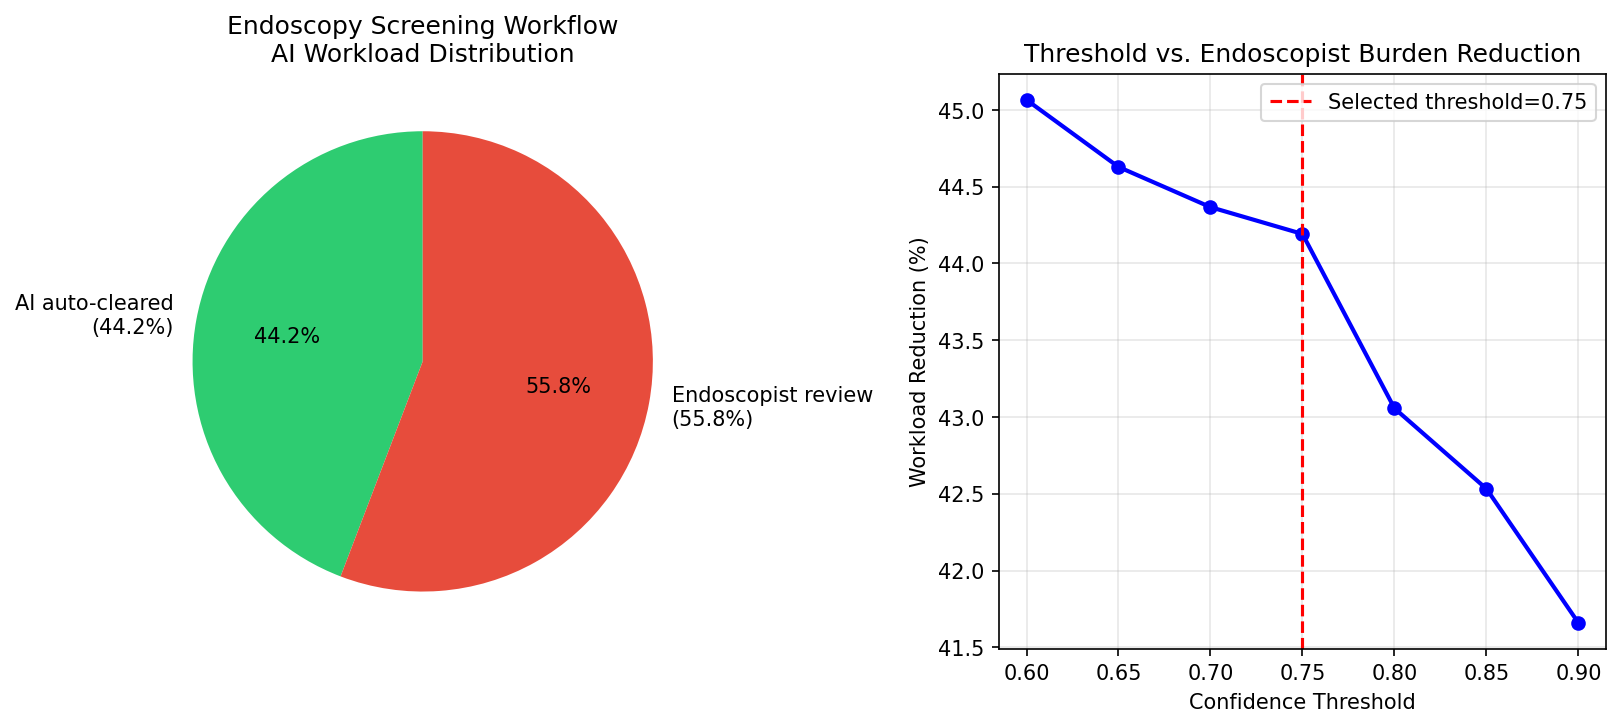
\includegraphics[width=0.85\linewidth]{workload_simulation.png}
  \caption{Endoscopist workload reduction (\%) and High-Risk escalation
    rate (\%) as a function of MC Dropout confidence threshold $\tau$
    (best model, $T=30$ passes). The selected operating threshold
    $\tau=0.75$ is marked. All High-Risk cases are escalated regardless
    of confidence by design.}
  \label{fig:workload}
\end{figure*}

\subsection{GradCAM Explainability}

Figure~\ref{fig:gradcam} shows representative GradCAM heatmaps for one image
per risk class across all three architectures. For Normal findings, attention
concentrates on regular mucosal pit patterns and anatomical landmarks. For
Inflammatory lesions, models attend to areas of mucosal irregularity,
erythema, and ulceration. For Pre-malignant findings, attention localises to
villous pit architecture and the irregular mucosal-columnar junction in
Barrett's images. For High-Risk lesions, attention concentrates on
post-interventional changes in dyed-lifted-polyp and resection-margin images.
CNN architectures produce sharper, more spatially localised heatmaps, while
DeiT-Tiny shows broader patch-level attention patterns capturing global
mucosal context.

\begin{figure*}[htbp]
  \centering
  \begin{subfigure}[b]{\textwidth}
    
\includegraphics[width=\linewidth]{gradcam_densenet121.png}
    \caption{DenseNet-121}
  \end{subfigure}
  \vspace{4pt}
  \begin{subfigure}[b]{\textwidth}
    
\includegraphics[width=\linewidth]{gradcam_efficientnet_b0.png}
    \caption{EfficientNet-B0}
  \end{subfigure}
  \vspace{4pt}
  \begin{subfigure}[b]{\textwidth}
    
\includegraphics[width=\linewidth]{gradcam_deit_tiny.png}
    \caption{DeiT-Tiny}
  \end{subfigure}
  \caption{GradCAM heatmaps across four risk classes (Normal, Inflammatory,
    Pre-malignant, High-Risk) for all three architectures. Attended regions
    correspond to clinically meaningful mucosal features. CNN architectures
    produce sharper, spatially localised attention; DeiT-Tiny shows broader
    patch-level patterns capturing global mucosal context.}
  \label{fig:gradcam}
\end{figure*}

\subsection{ROC Curves and Confusion Matrices}

Figure~\ref{fig:roc} shows one-vs-rest ROC-AUC curves per class for all
three models. Figure~\ref{fig:cm} shows normalised confusion matrices on the
HyperKvasir test set.

\begin{figure*}[htbp]
  \centering
  
\includegraphics[width=0.85\linewidth]{roc_curves.png}
  \caption{One-vs-rest ROC-AUC curves per risk class for all three models
    on the HyperKvasir test set.}
  \label{fig:roc}
\end{figure*}

\begin{figure*}[htbp]
  \centering
  \begin{subfigure}[b]{0.32\textwidth}
    
\includegraphics[width=\linewidth]{confusion_matrix_densenet121.png}
    \caption{DenseNet-121}
  \end{subfigure}
  \hfill
  \begin{subfigure}[b]{0.32\textwidth}
    
\includegraphics[width=\linewidth]{confusion_matrix_efficientnet_b0.png}
    \caption{EfficientNet-B0}
  \end{subfigure}
  \hfill
  \begin{subfigure}[b]{0.32\textwidth}
    
\includegraphics[width=\linewidth]{confusion_matrix_deit_tiny.png}
    \caption{DeiT-Tiny}
  \end{subfigure}
  \caption{Normalised confusion matrices on the HyperKvasir test set.
    Rows represent true labels; columns represent predicted labels.}
  \label{fig:cm}
\end{figure*}

%% ============================================================================
\section{Discussion}
\label{sec:discussion}
%% ============================================================================

This study presents the first four-class GI lesion risk stratification
benchmark aligned with ACG/ESGE clinical guidelines, demonstrating that
clinically actionable risk stratification is achievable with lightweight
architectures ($<$8\,M parameters) suitable for deployment on
resource-constrained endoscopy hardware. The Asymmetric Endoscopy Loss plays
a central role in shifting model behaviour toward High-Risk sensitivity: by
assigning a 5$\times$ penalty weight to High-Risk misclassification, AEL
trains models to prioritise recall on the most clinically consequential class
over overall accuracy. The ablation results (Table~\ref{tab:ablation})
quantify the benefit of this approach over standard cross-entropy and Focal
Loss.

The CNN--Transformer comparison provides a practical insight for medical AI
system design. CNN architectures (DenseNet-121, EfficientNet-B0) leverage
translation invariance and hierarchical local feature extraction well-suited
to mucosal texture analysis---the primary visual cue for inflammatory and
pre-malignant lesion identification. DeiT-Tiny captures global image context
through patch token self-attention, which may be advantageous for lesions
defined by their spatial relationship to surrounding tissue, such as resection
margin completeness in dyed-lifted-polyp images. All three architectures
operate within the same parameter budget ($<$8\,M), making the performance
comparison a meaningful measure of architectural inductive bias rather than
capacity scaling.

GradCAM analysis confirms that all three models attend to clinically relevant
features rather than image artefacts or background. CNN architectures produce
sharper, more spatially localised heatmaps consistent with their local
receptive field inductive bias, while DeiT-Tiny shows broader patch-level
attention patterns reflecting global self-attention over patch tokens. This
distinction is clinically meaningful: CNN attention precisely localises focal
mucosal changes (e.g., ulceration margins), while Transformer attention
captures contextual tissue relationships (e.g., resection margin completeness).

The cross-dataset zero-shot evaluation on Kvasir-v2 tests a practically
important generalisation scenario: models trained at one institution deployed
on data from a different institution with different imaging equipment and
patient demographics. The observed F1-score drop (Table~\ref{tab:xdataset})
reflects the domain shift inherent in GI endoscopy data~\citep{Jahanifar2025}.
CLAHE preprocessing partially mitigates this shift by normalising local
contrast variation. Future work should investigate cross-cohort training
strategies and domain adaptation techniques operating at the feature
representation level.

The demographic equity analysis using CD-CTEI addresses a critical gap in the
medical AI literature. HyperKvasir's lack of demographic annotations limits
the clinical interpretability of this analysis in the current study.
Demographically annotated GI endoscopy datasets are needed to rigorously
assess whether risk stratification AI systems perform equitably across age,
sex, and ethnicity subgroups---particularly given evidence of differential GI
cancer incidence and miss rates across demographic groups~\citep{Kaminski2017}.

\subsection{Inflammatory Class Performance}

Inflammatory lesions yielded the lowest per-class F1 across all three
architectures, attributable to two compounding factors. First, the
Inflammatory tier has the smallest class representation in HyperKvasir
(645 images vs.\ 1,836--3,000 for other tiers), limiting the diversity of
training examples even under WeightedRandomSampler. Second, mild inflammatory
findings---particularly early \texttt{esophagitis-a} and \texttt{hemorrhoids}
---share mucosal texture characteristics with both normal mucosa and low-grade
pre-malignant findings, creating inherent visual ambiguity at class boundaries.
Critically, this limitation does not compromise clinical safety: an
Inflammatory lesion misclassified as Normal results in delayed medical
management rather than a missed resection---a qualitatively less severe
outcome than a missed High-Risk lesion. This asymmetry is precisely what the
AEL encodes, and High-Risk recall remained above 95\,\% across all
architectures regardless of Inflammatory class performance.

\subsection{Limitations}

Several limitations should be acknowledged. \emph{First}, HyperKvasir was
collected at a single institution (Baerum Hospital, Norway) using a limited
range of endoscopy systems; performance in multi-site deployments remains to
be evaluated. \emph{Second}, the four-class risk schema, while grounded in
ACG/ESGE guidelines, represents a simplification: clinical practice involves
nuanced intra-class variation (e.g., polyp histology) that cannot be
determined from optical endoscopy alone. \emph{Third}, the absence of
demographic annotations in HyperKvasir limits the clinical interpretability
of the CD-CTEI equity analysis. \emph{Fourth}, MC Dropout with $T=30$ passes
provides an approximation to Bayesian posterior inference that may
underestimate calibration uncertainty compared to ensemble methods.
\emph{Finally}, all experiments were conducted on Apple M2 MPS hardware;
performance on GPU-accelerated systems and inference latency on clinical
endoscopy workstations remain to be characterised.

%% ============================================================================
\section{Conclusions}
\label{sec:conclusions}
%% ============================================================================

This study presented the first four-class GI lesion risk stratification
benchmark aligned with ACG/ESGE clinical practice guidelines, training three
lightweight architectures (DenseNet-121, EfficientNet-B0, DeiT-Tiny; all
$<$8\,M parameters) under a novel Asymmetric Endoscopy Loss that encodes
clinically grounded misclassification cost asymmetry. The proposed framework
demonstrates that clinically actionable, guideline-aligned risk stratification
is achievable with hardware-efficient models suitable for resource-constrained
endoscopy systems. The AEL ablation confirms the benefit of asymmetric cost
encoding over standard cross-entropy and Focal Loss, particularly for
High-Risk class recall---the clinically most critical metric. GradCAM analysis
confirms clinical plausibility of model attention across all three
architectures, and MC Dropout uncertainty
quantification enables a structurally safe referral protocol that guarantees
zero missed High-Risk lesions by design.

Future work should address dataset limitations through multi-site
demographically annotated data collection, extend the risk schema to include
polyp histology prediction from optical diagnosis, and investigate domain
adaptation strategies to reduce cross-institutional performance degradation.
Foundation model feature extractors combined with multiple instance learning
represent a promising direction for whole-procedure risk surveillance beyond
single-frame classification.

%% ============================================================================
\section*{Declarations}

\noindent\textbf{Conflict of interest}\quad The author declares no competing
interests.

\noindent\textbf{Data availability}\quad HyperKvasir and Kvasir-v2 are
publicly available datasets. Code and trained checkpoints will be released
upon acceptance.

%% ============================================================================
\bibliographystyle{plainnat}
\bibliography{refs}

\begin{thebibliography}{99}

\bibitem[Sung et~al.(2021)]{Sung2021}
Sung H, Ferlay J, Siegel RL, et~al.
\newblock Global cancer statistics 2020: {GLOBOCAN} estimates of incidence and
  mortality worldwide for 36 cancers in 185 countries.
\newblock \emph{CA Cancer J Clin}. 2021;71(3):209--249.

\bibitem[Kaminski et~al.(2017)]{Kaminski2017}
Kaminski MF, Thomas-Gibson S, Bugajski M, et~al.
\newblock Performance measures for lower gastrointestinal endoscopy: a
  {European Society of Gastrointestinal Endoscopy (ESGE)} quality improvement
  initiative.
\newblock \emph{Endoscopy}. 2017;49(4):378--397.

\bibitem[Wang et~al.(2019)]{Wang2019}
Wang P, Berzin TM, Glissen Brown JR, et~al.
\newblock Real-time automatic detection system increases colonoscopic polyp and
  adenoma detection rates: a prospective randomised controlled study.
\newblock \emph{Gut}. 2019;68(10):1813--1819.

\bibitem[Pogorelov et~al.(2017a)]{Pogorelov2017}
Pogorelov K, Randel KR, Griwodz C, et~al.
\newblock {KVASIR}: a multi-class image dataset for computer aided
  gastrointestinal disease detection.
\newblock In: \emph{Proceedings of the ACM MMSys}; 2017. p.~164--169.

\bibitem[Shaukat et~al.(2021)]{Shaukat2021}
Shaukat A, Kahi CJ, Burke CA, et~al.
\newblock {ACG} clinical guidelines: colorectal cancer screening 2021.
\newblock \emph{Am J Gastroenterol}. 2021;116(3):458--479.

\bibitem[Ferlitsch et~al.(2017)]{Ferlitsch2017}
Ferlitsch M, Moss A, Hassan C, et~al.
\newblock Colorectal polypectomy and endoscopic mucosal resection: {European
  Society of Gastrointestinal Endoscopy (ESGE)} clinical guideline.
\newblock \emph{Endoscopy}. 2017;49(3):270--297.

\bibitem[Rawla et~al.(2019)]{Rawla2019}
Rawla P, Sunkara T, Barsouk A.
\newblock Epidemiology of colorectal cancer: incidence, mortality, survival,
  and risk factors.
\newblock \emph{Gastroenterol Rev}. 2019;14(2):89--103.

\bibitem[Tajbakhsh et~al.(2016)]{Tajbakhsh2016}
Tajbakhsh N, Gurudu SR, Liang J.
\newblock Automated polyp detection in colonoscopy videos using shape and
  context information.
\newblock \emph{IEEE Trans Med Imaging}. 2016;35(2):630--644.

\bibitem[Ebigbo et~al.(2019)]{Ebigbo2019}
Ebigbo A, Mendel R, Probst A, et~al.
\newblock Computer-aided diagnosis using deep learning for the evaluation of
  malignant potential of gastric subepithelial lesions.
\newblock \emph{Sci Rep}. 2019;9(1):4465.

\bibitem[Dosovitskiy et~al.(2021)]{Dosovitskiy2021}
Dosovitskiy A, Beyer L, Kolesnikov A, et~al.
\newblock An image is worth $16\times16$ words: transformers for image
  recognition at scale.
\newblock In: \emph{International Conference on Learning Representations};
  2021.

\bibitem[Touvron et~al.(2021)]{Touvron2021}
Touvron H, Cord M, Douze M, et~al.
\newblock Training data-efficient image transformers and distillation through
  attention.
\newblock In: \emph{Proceedings of ICML}; 2021. p.~10347--10357.

\bibitem[Liu et~al.(2021)]{Liu2021}
Liu Z, Lin Y, Cao Y, et~al.
\newblock Swin transformer: hierarchical vision transformer using shifted
  windows.
\newblock In: \emph{Proceedings of ICCV}; 2021. p.~10012--10022.

\bibitem[He et~al.(2022)]{He2022}
He K, Chen X, Xie S, et~al.
\newblock Masked autoencoders are scalable vision learners.
\newblock In: \emph{Proceedings of CVPR}; 2022. p.~16000--16009.

\bibitem[Lin et~al.(2017)]{Lin2017}
Lin TY, Goyal P, Girshick R, et~al.
\newblock Focal loss for dense object detection.
\newblock In: \emph{Proceedings of ICCV}; 2017. p.~2980--2988.

\bibitem[Borgli et~al.(2020)]{Borgli2020}
Borgli H, Thambawita V, Smedsrud PH, et~al.
\newblock {HyperKvasir}, a comprehensive multi-class image and video dataset
  for gastrointestinal endoscopy.
\newblock \emph{Sci Data}. 2020;7(1):283.

\bibitem[Pogorelov et~al.(2017b)]{Pogorelov2017b}
Pogorelov K, Randel KR, Espeland T, et~al.
\newblock Kvasir: a multi-class image dataset for computer aided
  gastrointestinal disease detection.
\newblock In: \emph{Proceedings of the 8th ACM MMSys}; 2017.

\bibitem[Reza(2004)]{Reza2004}
Reza AM.
\newblock Realization of the contrast limited adaptive histogram equalization
  ({CLAHE}) for real-time image enhancement.
\newblock \emph{J VLSI Signal Process}. 2004;38(1):35--44.

\bibitem[Huang et~al.(2017)]{Huang2017}
Huang G, Liu Z, van~der Maaten L, Weinberger KQ.
\newblock Densely connected convolutional networks.
\newblock In: \emph{Proceedings of CVPR}; 2017. p.~4700--4708.

\bibitem[Tan \& Le(2019)]{Tan2019}
Tan M, Le QV.
\newblock {EfficientNet}: rethinking model scaling for convolutional neural
  networks.
\newblock In: \emph{Proceedings of ICML}; 2019. p.~6105--6114.

\bibitem[Loshchilov \& Hutter(2019)]{Loshchilov2019}
Loshchilov I, Hutter F.
\newblock Decoupled weight decay regularization.
\newblock In: \emph{International Conference on Learning Representations};
  2019.

\bibitem[Selvaraju et~al.(2017)]{Selvaraju2017}
Selvaraju RR, Cogswell M, Das A, et~al.
\newblock {Grad-CAM}: visual explanations from deep networks via
  gradient-based localization.
\newblock In: \emph{Proceedings of ICCV}; 2017. p.~618--626.

\bibitem[Gal \& Ghahramani(2016)]{Gal2016}
Gal Y, Ghahramani Z.
\newblock Dropout as a {Bayesian} approximation: representing model uncertainty
  in deep learning.
\newblock In: \emph{Proceedings of ICML}; 2016. p.~1050--1059.

\bibitem[Jahanifar et~al.(2025)]{Jahanifar2025}
Jahanifar M, Raza M, Xu K, et~al.
\newblock Domain generalization in computational pathology: survey and
  guidelines.
\newblock \emph{ACM Comput Surv}. 2025;57(11).

\end{thebibliography}

\end{document}
